% % % Set the style for this file:
\pagestyle{standard}

% % % Beginning of the chapter
\chapter{Infrared thermograms analysis}\label{chapter3}

	% % % Set the style for the first page:
	\thispagestyle{chapter-first-page}

	\section{Apparent reflected temperature estimation.}\label{section3.1}
	
		In order to correctly estimate the emissivity of any surface, it is very important to determine first the surface apparent reflected temperature. This is crucial, especially for low emissivity materials where a significant contribution is in fact the reflected radiation.
		
		A simple method can be used to determine the apparent reflected temperature. To do it, a low emissivity material is needed, usually, an aluminum foil or any other aluminum surface. This method is described as follows:
		
		\begin{enumerate}[label={\arabic*)}]
			\item Place a piece of crumpled and re-flattened aluminium foil in the same position of the object to be measured.
			\item Set the IR camera emissivity internal control to 1.00 and the distance to 0 m.
			\item Point the IR camera to the target (aluminum surface) and select a region of interest (ROI).
			\item Read the value from IR camera on the ROI.
			\item Take the measured value as the apparent reflected temperature.
		\end{enumerate}
	
		Aluminum foil has very low emissivity ($\sim$0.04) and therefore we are certain that almost all IR radiation coming from the surface is reflected from other sources. The camera emissivity is set to 1.00 and the distance to 0 so that the IR camera software does not apply any further correction. The crumpling is done to allow reflections from several directions, for this reason the ROI selected should be as wide as possible since this effect must be averaged out to obtain an accurate estimate of the apparent reflected temperature.\bigskip
	
	\section{IR camera spectral response.}\label{section3.2}
	
		From Equation \ref{eq1.16} it can be seen that if we can accurately estimate the emissivity, the apparent reflected temperature and the IR camera spectral response function ($R$) we should be able then to obtain the real temperature of the object for any given spectral power value reported by the camera ($N_{meas}$). 
		
		In order to estimate the $R$ factor we can simply take the emissive power measurements of a surface of known emissivity, the real temperature and the apparent reflected temperature and then use the same Equation \ref{eq1.16} to derive the $R$ scale factor. As this factor only depends on the IR camera, it can be used later on in the analysis as long as we don’t use a different camera.
		For obtaining the scale factor we used an aluminum bucket which we filled with hot water and recorded the IR power density on several points of the surface (always at the same depth). The measured aluminum surface was coated with high emissivity black\footnote{{\footnotesize Note that the "visible" color of the tape has nothing to do with the emissivity value. It could have been a red, green or even white. The color of the tape is a property related with the visible wavelengths in electromagnetic spectrum while the infrared properties are related with the IR part of the spectrum.}} tape as the water temperature went down to test the temperature dependence of the results (Figure \ref{fig3.1}).
		
		\begin{figure}[ht!]
			\centering
			\captionsetup{justification=centering,margin=2cm}
			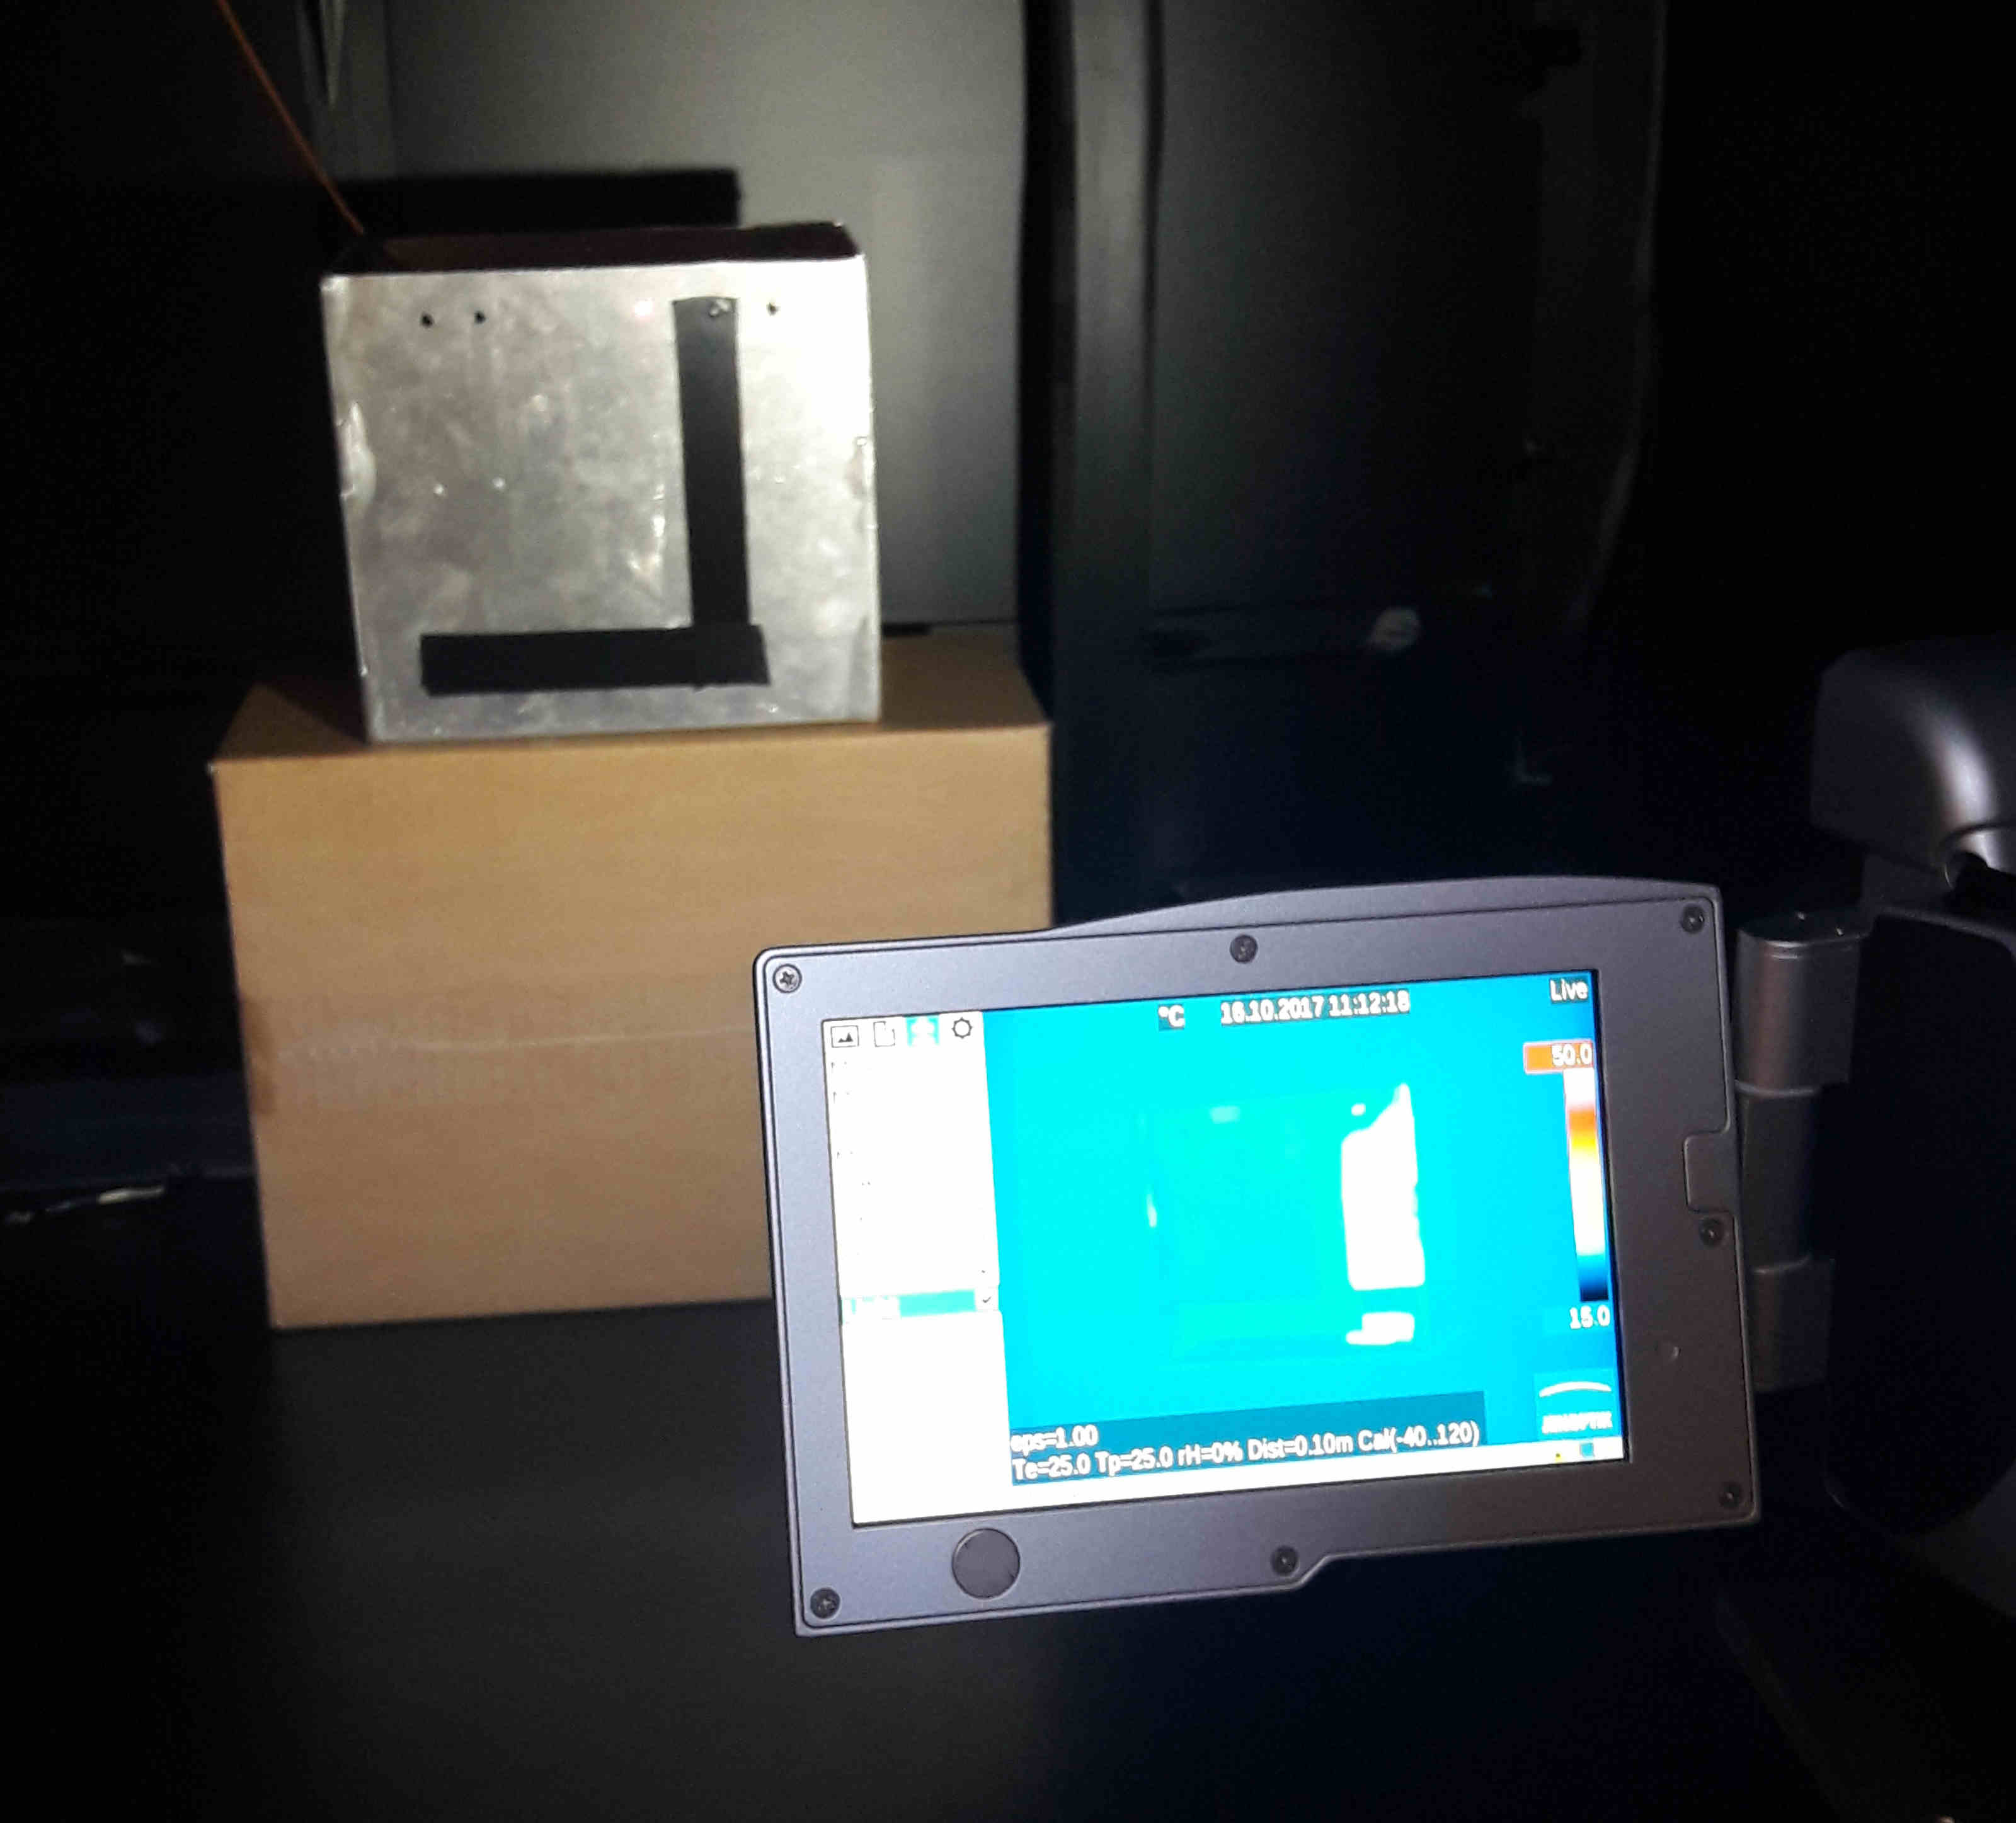
\includegraphics[scale=0.10]{Figures/Chapter03/CameraAndBucket.jpg}
			\caption{Experimental setup to calculate the IR camera spectral response function. Measurements were performed placing height measurement markers along the horizontal black tape in the camera IRBIS software.}\label{fig3.1}
		\end{figure}
		
		With this scale factor and Equation \ref{eq1.16} we could estimate the emissivity at pixel level if we had a thermogram in which the real temperature of all the pixels is known. That would allow correct the thermograms in emissivity without the need of covering the Silicon surfaces with high emissivity materials (See Section \ref{section3.3}). In the next section we will refer to this method as the “baseline image” method.\bigskip
		
	\section{Emissivity estimation. }\label{section3.3}
		
		As the main source of discrepancies comes from the differences in emissivity, this is very often the starting point for IR image calibration. Almost all IR cameras can be set to a certain value of emissivity (usually set to 1.00 by default). If we knew the emissivity value of certain surface we could then enter that value into the IR camera software and the apparent temperature, i.e. temperature displayed by the IR camera, would be close to the real temperature. This is what we would call a “direct” emissivity correction method. It is of course the most simple but also the most uncommon way to correct an IR image for more complicated quantitative studies. On one side, we usually don’t know beforehand the emissivity value of the surface we want to measure and, on the other side, this method would only give us the correct temperature on the surface of known emissivity.
		
		There are also some other ways to calculate the emissivity of a surface. One of them consists in estimating the surface’s emissivity by using an alternative temperature measurement as reference. With that purpose, the following method can be used  \ref{ref11}, \ref{ref12}:
		
		\begin{enumerate}[label={\arabic*)}]
			\item Measure the surface temperature by an alternative method (thermocouple, known emissivity coating).
			\item Set the necessary measurement parameters (ambient temperature, RH, distance to target, ...) in the IR camera software as needed and the emissivity to 1.
			\item Point the IR camera to the target and select a region of interest (ROI).
			\item Modify the value of emissivity in the camera software until the apparent temperature in the selected ROI equals the one measured with the alternative method. This is the emissivity of the target surface.
			\item Repeat steps 2) to 4) as many times as necessary to minimize the measurement uncertainty.
		\end{enumerate}
	
		Using this approach a “global” IR image emissivity correction can be applied to get temperature values close to the real ones on the silicon surface. However, as mentioned before, this will only show accurate readings in those areas corresponding to the surface of estimated emissivity. The rest of the elements in the image that have different emissivity values might appear to have a complete different temperature of what they actually have. However, if we are not interested in the whole picture but just in one particular material in it, this simple method can be very useful. The problems begin when the surface of interest has relatively low emissivity. In such cases temperature estimation may not be very accurate because low emissivities are hard to estimate and small changes in their values can lead to large variations in the temperature measurements \ref{ref13}. In other words, the lower the emissivity of the surface, the bigger the uncertainty associated with it \ref{ref14}.
		
		Another approach consists in using a “relative” method exploiting the Equation \ref{eq1.16}. Let's imagine that we have two surfaces at the same temperature, then, if we apply Equation \ref{eq1.16} on the one that we know the emissivity value (e.g. black tape) and on the one we want to estimate it from (e.g. silicon surface) then we obtain:
		
		\begin{equation}\label{eq3.1}
			N^{BT}_{meas}(T_{BT})= R \cdot \bar{\varepsilon}_{BT} \cdot I_{1}(T_{BT}) + R \cdot [1- \bar{\varepsilon}_{BT}] \cdot I_{2}(T_{r})
		\end{equation}
			
		\begin{equation}\label{eq3.2}
			N^{Si}_{meas}(T_{BT})= R \cdot \bar{\varepsilon}_{Si} \cdot I_{1}(T_{BT}) + R \cdot [1- \bar{\varepsilon}_{Si}] \cdot I_{2}(T_{r})
		\end{equation}\bigskip
	
		Here $T_{BT}$ is the apparent (measured with the IR camera) temperatures of the black tape. Note that as the “real” temperature we have selected the apparent temperature of the black tape. We can do so since the black tape has high emissivity and therefore the IR camera should give accurate temperature readings without any further correction. Naturally we know that $N^{BT}_{meas}(T_{BT}) \neq N^{Si}_{meas}(T_{BT})$, however, we can use a small trick here: as the black tape has high emissivity, if we replace $T_{BT}$ in Equation \ref{eq3.1} with the apparent temperature of the silicon ($T_{Si}$) then $N^{BT}_{meas}(T_{Si}) = N^{Si}_{meas}(T_{BT})$. This is equivalent to say that we have measured a "real" temperature equal to $T_{Si}$ in then surface covered by black tape. After rearranging terms we obtain:
		
		\begin{equation}\label{eq3.3}
			\bar{\varepsilon}_{Si} = \bar{\varepsilon}_{BT} \cdot \frac{I_{1}(T_{Si}) - I_{2}(T_{r})}{I_{1}(T_{BT}) - I_{2}(T_{r})}
		\end{equation}\bigskip
	
		Note that this expression is invalid if the silicon surface is considerably transmissive, since we have neglected transmissivity for deriving Equation \ref{eq1.16}, and when the real temperature ($T_{BT}$) is close to $T_{r}$ in which case Equation \ref{eq3.3} does not hold anymore. This is known as the “black tape method” and, as the name indicates, consists in covering the surface of interest with a material of known emissivity (usually high emissivity) and use the direct correction method on the coated surface.
		
		For the Petal’s thermal study, parts of the silicon surface on both sides were covered with high emissivity black tape (Figure \ref{fig3.2}). The black tape used for this setup has an emissivity of 95\% and therefore the coated surface will behave almost like a blackbody. 
	
		\begin{figure}[ht!]
			\centering
			\captionsetup{justification=centering,margin=2cm}
			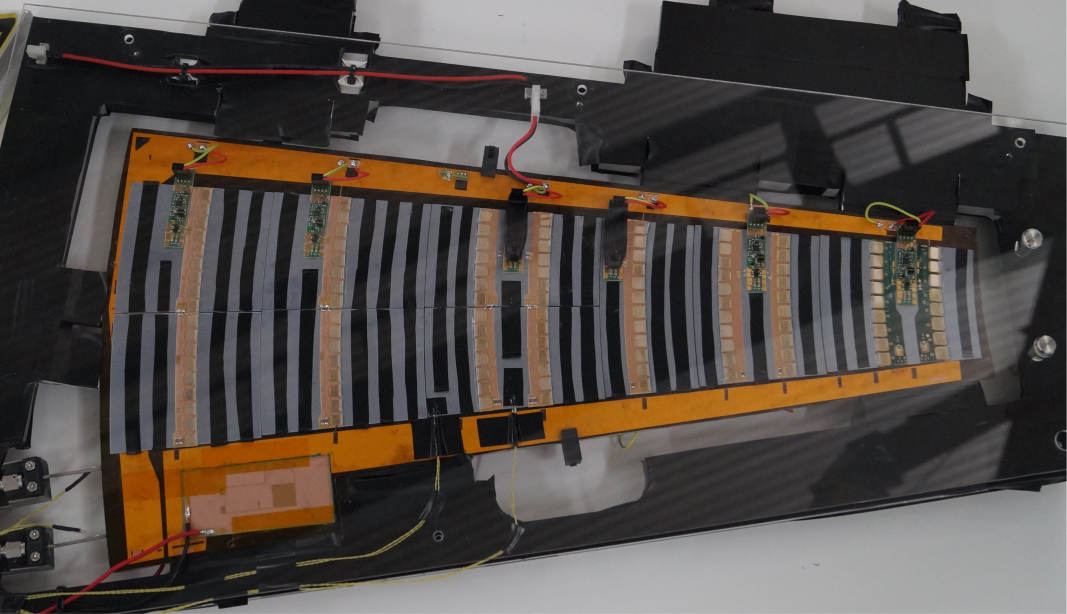
\includegraphics[scale=0.40]{Figures/Chapter03/ZebraPetal.jpg}
			\caption{Unpolished side of the “Zebra” Petal covered with stripes of black electrical tape of high emissivity.}\label{fig3.2}
		\end{figure}
	
		For our black taped petal (“zebra”), setting the IR camera emissivity to 0.95 (95\%) allows us to measure an apparent temperature very close to the real temperature. This is true if we assume that both the surface of interest and the black tape on top of it have reached thermodynamic equilibrium. Using the IRBIS software a set of over 560 measurement markers (ROIs) were created on the black tape strips to create a map of corrected temperatures. Additionally, a set of markers was created on the silicon surface right next to the corresponding black tape marker to be able to estimate the emissivity of the silicon using the black tape markers readings as the “real” temperature values. With this method we could perform calibrated temperature measurements on the Petal’s silicon surface to be able to compare with FEA simulations (See Chapter \ref{chapter4}). However, as it can be seen from the picture, we had to add adhesive material onto the silicon surface, which would be unacceptable during production stages for quality control. 
		
		Let’s now discuss another method, known as the “baseline image” method. Let's we assume that we have a thermogram of which we know the real temperature of all the pixels. That could be, for example, a thermogram of the Petal at room temperature (Figure \ref{fig3.3}). The fact that we still see differences of temperature in the image even though everything is at the same temperature is evidence (to a first approximation) of the effect of the different emissivity values of the materials composing the Petal. We call such image a baseline thermogram. The advantage of the baseline thermogram is that we know the real temperature of all the pixels beforehand and therefore we could use Equation \ref{eq1.16} to calculate the emissivity of each pixel. 
	
		\begin{figure}[ht!]
			\centering
			\captionsetup{justification=centering,margin=2cm}
			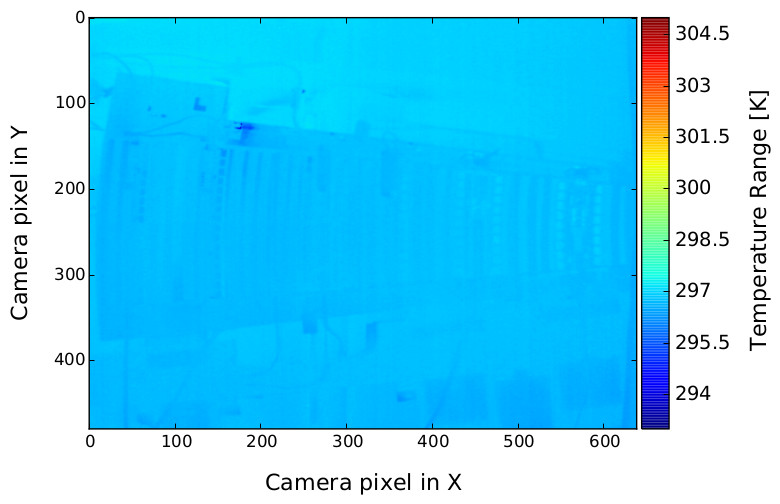
\includegraphics[scale=0.55]{Figures/Chapter03/thermo_Temp_201708091701_avg.jpg}
			\caption{Thermogram of the petal at room temperature (not powered and no CO2 flushed in). Even though everything is at the same temperature, we still can see the shape of the petal.}\label{fig3.3}
		\end{figure}
	
		This method, however, presents an associated difficulty: if the baseline is at room temperature, it means that we can not use Equation \ref{eq1.16} directly to obtain emissivity but, instead, we can use it iteratively to estimate emissivity to some degree of accuracy. Of course this makes even worse the errors in the estimation of emissivity but it’s the price to pay for not touching the petal. The other important disadvantage is that, in order to be able to extrapolate the values of emissivity calculated on the baseline image to other thermograms we must be sure that the camera does not move in between, otherwise the pixels won’t match anymore and the emissivity values would not be valid.
		
		Finally, we have also assumed that the emissivity does not depend on the surface temperature under the graybody approximation, which is not true in general. However, except for the case of selective emitters, emissivity is a very slowly-variating function of the surface’s temperature.
		
		The fact that the dummy silicon sensors in the front (polished) side of the petal are highly transmissive (See Chapter \ref{chapter4}), together with the aforementioned difficulties, made it impossible\footnote{{\footnotesize This automatically invalidates Equation \ref{eq1.16} since transmission was ruled out in its derivation}} for us to use this emissivity correction method for the present study. Instead, the "zebra" petal approach, using the IRBIS set of ROI markers on the black tape strips was used for obtaining comparable results to FEA simulations.\bigskip
		
	\section{Influence of the angular distribution of the emitted IR radiation.}\label{section3.4}
	
		In order to determine whether the viewing angle of the camera with respect to the normal of the petal's surface is a determining factor in our analysis, an study of the angular dependence of emissive power was performed using an aluminum rod filled with hot water placed in the same position as the Petal. Using a strip of high emissivity black tape along the rod’s frontal face we were able to measure the variations in temperature due to the viewing angle (Figure \ref{fig3.4}).
	
		\begin{figure}[H]
			\centering
			\captionsetup{justification=centering,margin=2cm}
			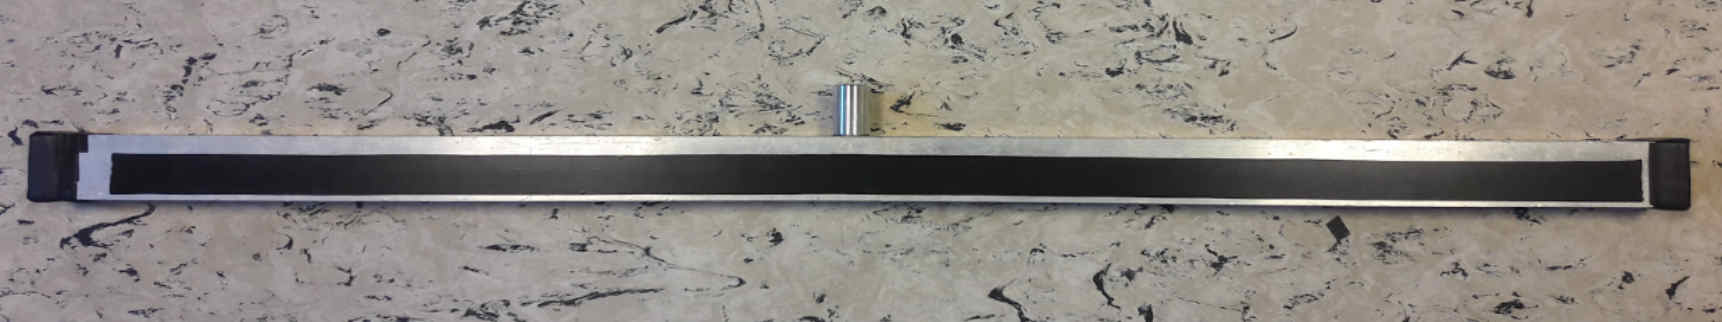
\includegraphics[scale=0.30]{Figures/Chapter03/AluminumRod.jpg}
			\caption{Aluminum rod used to study the angular dependence of emissivity}\label{fig3.4}
		\end{figure}		
		
		A set of measuring areas (ROI) was defined along the rod using the IR camera software (IRBIS) and a thermocouple was inserted inside the rod in direct contact with the water in order to be able to determine the real temperature of the rod surface.
	
	